\chapter{Практическая часть}
\label{cha:ch_2}


При выборе базового фреймворка для реализации функциональности, описанной в теоретической части следовало опираться на следующие факторы:

\begin{itemize}
    \item Открытый и понятный исходный код с лицензией, позволяющей добавление собственного программного кода.
    \item Наличие собственного формата in-memory представления нейронной сети.
    \item Наличие формата и инструментов для сериализации/десериализации глубоких моделей.
    \item Наличие легковесного интерпретатора для нейронных моделей, который можно расширить добавлением собственных вычислительных ядер для интерпретации новых нейронных слоёв. 
    \item Наличие инструментов, которые позволяют переводить глубокие модели во внутренний формат из других популярных форматов, в которых могла быть обучена исходная нейронная сеть.
\end{itemize}

Среди проектов, соответствующих выделенным критериям, ярко выделяются такие, как Tensorflow от компании Google и ONE от компании Samsung. Выбор был сделан в пользу последнего, поскольку он активно развивается под лицензией Apache 2.0, а его интерпретатор показывает лучшие результаты в проведенных бенчмарках на ЭВМ с жесткими ограничениями в ресурсах за счет лучшей работы с памятью.

Разработка велась в локальном форке исходного проекта на GitHub в отдельной ветке (URL: https://github.com/Bronnikoff/ONE/tree/lq\_nets), поскольку это удобный способ управлять добавляемым кодом при определенной независимости от параллельных изменений, вносимых в базовый проект со стороны его разработчиков.

\section{Поддержка слоя в графовых представлениях}

Квантизованный слой имеет отличное от оригинального слоя поведение при вычислениях, количество параметров и формат хранения данных. Это означает, что для поддержки его работы и для удобства обработки графа при написании квантизатора, необходимо поддержать новую операцию LQFullyConnected во всех имеющихся в ONE графовых представлениях, которые используются для работы с моделью от этапа её считывания из файла до этапа расчета результатов ее работы. Префикс LQ (Learnable Quantization), содержащийся в названии операции, был добавлен к названию чтобы указать на то, что она является результатом перевода полносвязанного (FullyConnected) слоя в низкобитовый формат при помощи обучаемых параметров квантизации.


Такими графовыми представлениями, через которые проходит модель до непосредственного запуска, являются:
\begin{itemize}
    \item Представление circle для сериализации и десериализации графовых моделей с жёсткого диска.
    \item In-memory представление luci, которое работает со слоями как с вершинами, соединенными друг с другом посредством указателей.
    \item Вычислительный граф, который оперирует тензорами, связанными друг с другом вычислительными ядрами операций.
\end{itemize}

Реализацию было решено начать с описания схемы хранения квантизованного слоя в долгосрочной памяти  вместе со схемой его сериализации и десериализации (способа записи структуры данных на жесткий диск и извлечения её из него). Благодаря тому, что принятый в Samsung формат хранения моделей circle основан на известной технологии flatbuffers, этот этап потребовал лишь описания в файле circle-schema.fbs параметров, которые уникальны и присущи только добавляемому слою. 

\begin{lstlisting}[language=C++, caption={Структура слоя в схеме}]
table LQFullyConnectedOptions {
	hidden_size: int;
	fused_activation_function:ActivationFunctionType;
}
\end{lstlisting}

Этими параметрами являются тип функции активации, которая применяется к выходу сумматора каждого нейрона и число hidden\_size, равное размеру входного вектора, поскольку его необходимо знать в случаях, когда размер входных данных не делится на цело на 32, для корректного расчета бинарных скалярных произведений при работе операции.

Помимо описания уникальных параметров LQFullyConnected, требуется декларировать наличие этого нового оператора и присвоить ему уникальный номер в схеме формата circle, который был выбран случайным образом.

Остальная работа по сохранению и извлечению модели производится самим flatbuffers. При помощи компилятора flatc, предоставляемого компанией Google, на основе схемы, которая была расширена параметрами нового слоя, генерируется хедер-файл для языка С++. Этот файл schema\_generated.h реализовывает алгоритм перевода набора байт из дискового пространства в описанную в С++ структуру хранения этой операции в памяти при работе программы, извлекая в том числе и информацию о связях с соседними операциями в графе модели. Стоит отметить, что flatc поддерживает несколько языков программирования, таких как Java или JS, а не только C++, что позволяет работать с circle не только в C++. Применение этого свойства будет показано далее.

После того, как новая операция была добавлена в circle, следует перейти к поддержке LQFullyConnected в основном промежуточном представлении (Intermideate Representation) под названием luci. В отличие от 2-ух других представлений, оно не создано для решения какой-то конкретной задачи, такой как высокопроизводительный запуск сети или реализация алгоритмов работы с сырыми данными из файла. Поэтому в нём модели представлены в виде классических графов, вершинами которых являются операции, а связи между соседними слоями прописаны явно, через указатели языка C++. Универсальный вид графа делает его удобным для применения различных оптимизаций с подграфами модели. Также из него удобно перевести модель в любой другой формат, который заточен под решение конкретной задачи.

Следует выделить 4 основных части в формате luci:
\begin{enumerate}[label=\arabic*.]
    \item Описание представления каждой операции в формате. (luci/lang)
    \item Функциональность для импорта модели из circle. (luci/import)
    \item Функциональность для экспорта модели из circle. (luci/export)
    \item Алгоритмы оптимизации, применяемые к графу. (luci/pass)
\end{enumerate}

На уровне описания структуры представления LQFullyConnected в luci, отраженной на листинге 2.2, явно объявляется, что новая операция должна иметь 5 входных вершин: входная вершина, из которой поступают входные данные, базис-вектор для квантизации входных данных, набор базис-векторов для квантизации весов слоя, бинаризованные веса и вектор смещений.

\begin{lstlisting}[language=C++, caption={Структура слоя в luci}]
class CircleLQFullyConnected final : public FixedArityNode<5, 
    CircleNodeImpl<CircleOpcode::LQ_FULLY_CONNECTED>>,
    public CircleNodeMixin<CircleNodeTrait::FusedActFunc>,
    public CircleNodeMixin<CircleNodeTrait::Bias>
{
public:
  loco::Node *input(void) const { return at(0)->node(); }
  void input(loco::Node *node) { at(0)->node(node); }

  loco::Node *input_scales(void) const { return at(1)->node(); }
  void input_scales(loco::Node *node) { at(1)->node(node); }

  loco::Node *weights_scales(void) const { return at(2)->node(); }
  void weights_scales(loco::Node *node) { at(2)->node(node); }

  loco::Node *weights_binary(void) const { return at(3)->node(); }
  void weights_binary(loco::Node *node) { at(3)->node(node); }

  loco::Node *bias(void) const override { return at(4)->node(); }
  void bias(loco::Node *node) override { at(4)->node(node); }

public:
  int32_t weights_hidden_size(void) const { 
    return _weights_hidden_size; 
  }
  void weights_hidden_size(int32_t weights_hidden_size)
  {
    _weights_hidden_size = weights_hidden_size;
  }

private:
  int32_t _weights_hidden_size = 0;
};
\end{lstlisting}

Стоит отметить, что luci явно не требует, чтобы все из входных вершин существовали. Например, bias() может принимать значение nullprt. 

Основная функциональность для перевода моделей из luci в circle и обратно уже была реализована внутри проекта профессионалами из Samsung, что потребовало тривиальных изменений в исходном коде для поддержки импорта и экспорта.

Оптимизации для подграфов, содержащих LQFullyConnected в данной работе не рассматриваются, поэтому единственные алгоритмы, которые потребовалось реализовать в luci/pass — это определение типа данных (TypeInferencePass) и алгоритм определения размерности выходов слоя на основе размеров входных вершин (ShapeInferencePass).

Опциональной частью этой работы стала модификация существующего в проекте кода, отвечающего за отображение свойств операции в текстовом формате. Помимо этого, было полезно иметь наглядную визуализацию сетей, в графе которых присутствует добавляемая в этой работе операция. Для этого был модифицирован исходный код другого популярного проекта для визуализации множества различных нейросетевых форматов netron, который работает на языке JS. Как было отмечено ранее, flatc умеет переводить схему не только в C++, но и в JS. Сгенерированная с помощью flatc в JS схема работы с форматом circle была добавлена в этот инструмент, а остальная функциональность для работы с этой схемой уже присутствовала в «исходниках» визуализатора, поскольку он уже поддерживает формат tflite, который также основывается на flatbuffers.

При помощи описания простой нейронной сети с одним входом, одной LQFullyConnected операцией и одним выходом, при использовании имеющегося в проекте ONE инструмента circlechef для перевода описаний моделей в реальные физические модели, был получена первая сеть, визуализация которой netron-ом дала результат на рис. 2.1.

\begin{figure}[H]
    \begin{center}
        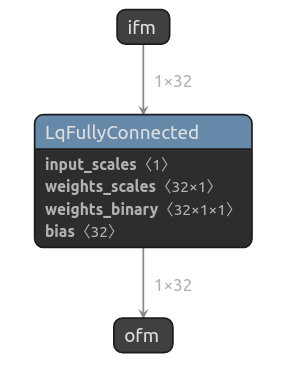
\includegraphics[scale=0.4]{tex/inc/img/lq.png}
        \caption{Пример модели с LQFullyConnected}
    \end{center}
\end{figure}

Возможность анализа моделей посредством визуализатора не входит в данную работу как необходимая ее часть, однако позволяет увеличить удобство работы пользователя с сетями в формате circle и ускорить дальнейший процесс разработки и отладки кода.

Последним из выделенных графовых представлений является форма вычислительного графа, которая спроектирована таким образом, чтобы минимизировать издержки при работе с слоями и достичь максимальной производительности. Вершинами в этом представлении являются тензоры, связанные между собой вычислительными ядрами. Для того, чтобы поддержать операцию на этом уровне, необходимо определить класс для операции, инкапсулирующий в себе разные вычислительные ядра в зависимости от типа поступающих данных и описывающий логику взаимодействия тензоров между собой.

Такой класс помимо ядер и указателей на входные и выходные тензоры содержит метод configure(), который необходимо переопределить для:

\begin{itemize}
    \item Проверки, что со входными тензорами можно провести запуск ядра. Именно в этом месте накладываются ограничения на параметры квантизованного слоя, описанные и обоснованные в теоретической части этой работы.
    \item Определения размерности данных, с которыми необходимо оперировать вычислительному ядру, и аллоцирования выходного тензора.
    \item Создания и инициализация вспомогательных вычислительных структур. Здесь создается объект класса LQBinarizer, инкапсулирующий в себе квантизацию входных данных вместе буфером для его квантизованных значений.
\end{itemize}

\section{Вычислительное ядро интерпретатора}

Вычислительное ядро интерпретатора вычисляет выходы операции LQFullyConnnected на основе входных данных, находящихся в тензоре input. Поскольку поступающие входные данные являются вещественными, а не квантизованными, перед расчетом выхода отдельного нейрона для одного входного вектора по формуле (1.8) необходимо произвести квантизацию входного вектора, с целью получения закодированного int32 буфера, который будет использоваться при расчетах. В связи с этим следует рассмотреть 2 основные части, которые требуется реализовать для поддержки корректной работы интерпретатора с моделями, содержащими LQFullyConnected:

\begin{itemize}
    \item Класс LQBinarizer, позволяющий проводить кодирование входных вещественных векторов и предоставляющий доступ к бинарным данным.
    \item Функция evalFloat, производящая расчет выходов по формуле (1.8), используя LQBinarizer внутри себя.
\end{itemize}

\subsection{Кодировщик LQBinarizer}

Для квантизации входных значений <<на лету>> появилась необходимость ввести вспомогательный класс LQBinarizer, объявление которого показано на листинге 2.3.

\begin{lstlisting}[language=C++, caption={Класс кодировщика}]
class LQBinarizer
{
  using Level = std::pair<float, int32_t>;

public:
  LQBinarizer(int32_t data_vec_size, const Tensor *data_scales);

  const int32_t *data() { return data_binary.get(); }

  void quantize_and_pack(const float *data_vector);

private:
  int32_t bin_search_encoding(float value);

private:
  int32_t data_float_size;
  int32_t data_bin_size;
  int32_t encode_bits;
  std::unique_ptr<int32_t[]> data_binary;

  int32_t levels_count;
  std::unique_ptr<Level[]> quantization_levels;
  std::unique_ptr<float[]> quantization_thresholds;
};
\end{lstlisting}

В конструкторе класса определяются пороги и уровни квантизации в отсортироанном порядке. Они необходимы для определения оптимальной кодировки для каждого из вещественных чисел. Помимо этого, при создании объекта класса происходит аллокация буфера бинарных данных и определяется чило $data\_bin\_size = ceil(data\_float\_size / 32)$, которое равно длине одной строки выделенного буфера. Было решено сделать выделение памяти за один раз в конструкторе, связав её освобождение с концом жизни объекта кодировщика через умные указатели, чтобы снизить издержки на ее перевыделение при расчете квантизованных значений во время работы вычислительного ядра. 

Метод quanitize\_and\_pack тривиально проходит по переданному ему вектору данных, который должен быть фиксированной длины data\_float\_size, и заполняет в соответствующую строку буфера data\_binary биты числа, полученного вызовом приватного метода bin\_search\_encoding. 

Метод bin\_search\_encoding является модифицированной версией классического бинарного поиска по массиву порогов $t$. Для любого поступаемого на вход значения $x: t_l < x \leq t_{l + 1}$, он возвращает число $l$. После чего, используя число $l$ в качестве индекса в массиве упорядоченных порогов, определяется оптимальная кодировка для числа $x$.

\subsection{Расчет выходов слоя}

В методе evalFloat по формуле (1.8), реализованной кодом с листинга 2.4, рассчитываются выходы нейронов для каждого из входных векторов. 

\begin{lstlisting}[language=C++, caption={Расчет выходов слоя}]
// calculate over output float values
for (int32_t bi = 0; bi < input_encode_bits; ++bi)
{
  // input computation data
  float inp_s = input_scales_data[bi];
  int32_t *inp_bin_line = &input_binary_data[bi * real_size];

  for (int32_t bw = 0; bw < weights_encode_bits; ++bw)
  {
    int32_t w_offset = calcOffset(weights_scales_shape, out_idx, bw);
    float w_s = weight_scales_data[w_offset];
    int32_t *w_bin_line = &weights_binary_data[w_offset * real_size];

    // add to total
    output_total += inp_s * w_s * bin_dot(inp_bin_line, w_bin_line);
  }
}
output_data[calcOffset(out_shape, batch, out_idx)] = output_total;
\end{lstlisting}

Расчёт бинарного скалярного произведения выполняется лямбда-выражением с листинга 2.5 при помощи побитовых операций и внутренней функции компилятора gcc \_\_builtin\_popcount, которая понижается при компиляции с опцией -mpopcnt в соответствующую ассемблерную инструкцию POPCNT из набора команд SSE4.2 для процессоров Intel.

\begin{lstlisting}[language=C++, caption={Бинарное скалярное произведение}]
auto bin_dot = [hidden_size, real_size]
(const int32_t *data_1, const int32_t *data_2) {
  int32_t positives = hidden_size - (real_size << 5); // hs - 32*rs
  for (int32_t i = 0; i < real_size; ++i)
  {
    positives += __builtin_popcount(~(data_1[i] ^ data_2[i]));
  }
  return (positives << 1) - hidden_size; // 2*positives - neurons_count
};
\end{lstlisting}

Недостатком такой реализации является возможное отсутствие поддержки \_\_builtin\_popcount в компиляторах, отличных от gcc. Эта проблема должна быть решена с переходом проекта ONE со  стандарта C++14 на C++20, в котором присутствует функция std::popcount.

\section{Квантизатор}

Для того, чтобы использовать нейронные сети с квантизованныи полносвязанными нейронными слоями для решения реальных задач, поддержки LQFullyConnected в интерпретаторе и графовых представлениях недостаточно. Данная работа не имеет смысла без инструмента, который переводил бы уже обученные нейронные сети в квантизованный формат с подбором оптимальных параметров и бинарных весов для каждого из FullyConnected слоёв. Поэтому в рамках этой работы вводится и описывается подобный инструмент, получивший название lquantizer. Его работа основана на следующих этапах:
\begin{enumerate}[label=\arabic*.]
    \item Считывание исходной нейронной сети  fp\_graph и создание ее копии lq\_graph - результата работы инструмента, которая будет изменяться в процессе работы lquantizer.
    \item Проход по соответствующим вершинам 2-ух сетей с целью:
    \begin{itemize}
        \item Замены в результирующей сети всех FullyConnected слоев на LQFullyConnected.
        \item Определение входных вершин соответствующих слоев обоих сетей для дальнейшего использования при обучении.
    \end{itemize}
    \item Обучение параметров квантизации для каждой из вершин LQFullyConnected.
    \begin{itemize}
        \item Обучение весовых параметров в lq\_node на основе соответствующего массива весов из fp\_node.
        \item Обучение квантизаторов lq\_node по входным значениям fp\_node с целью минимизации ошибки с входными значениями fp\_node.
        \item Дообучение квантизаторов lq\_node по входным значениям lq\_node с целью минимизации ошибки с входными значениями fp\_node. 
    \end{itemize}
\end{enumerate}

Особый интерес среди указанных выше шагов представляет основной этап программы: обучение параметров.

\subsection{Поиск оптимальных значений}

Для поиска оптимальных параметров квантизации как для весов, так и для входов слоя, был создан класс QEM(Quantization Error Minimization), реализующий в себе итеративное обучение по предложенному в теоретической части алгоритму. В нем используется расширенный класс LQBinarizer из интерпретатора. В этот класс добавлен метод gradient\_descent\_scales, который принимает массив данных, с которыми требуется минимизировать ошибку, и ищет оптимальные значения для базис-вектора по формуле (1.14) на основе текущей матрицы бинарных кодировок. Стоит напомнить, что LQBinarizer обладает методом quantze\_and\_pack, который заполняет внутренний буфер кодировками, являющимися оптимальными для текущего базис-вектора. Сам метод QEM итеративно вызывает методы gradient\_descent\_scales и quantize\_and\_pack указанное число раз и заботится об упорядоченности базис-вектора.

\subsection{Обучение весовых параметров}

Для того, чтобы обучить весовые параметры каждого слоя, необходимо пройти по соответствующим вершинам lq\_graph и fp\_graph и для каждого из нейронов в них вызвать QEM::fit() для поиска оптимальных значений параметров квантизации. Поскольку для весов следует хранить не только параметры квантизации, но и бинарные данные, следует закодировать веса из fp\_node полученными параметрами квантизации, используя объект класса LQBinarizer, что делает метод QEM::fill\_binary().

\subsection{Обучение и дообучение входных параметров}

\subsubsection{Сохранение входных значений}

Поскольку ONE является высокопроизводительным фреймворком для запуска сетей, но не для их обучения, добавить  в существующую архитектуру возможность сохранения входных значений для каждого из квантизуемых слоев с целью использования их для поиска оптимального распределения уровней квантизации, стало непростой задачей. 

luci\_interpreter позволяет реализовать и передать ему соответствующий обработчик Observer, который будет вызываться интерпретатором после завершения каждого из ядер. Обработчик может получать указатель на вершину соответствующей операции в luci графе и на тензор с выходными значениями, полученный в результате исполнения ядра.

Поэтому для того, чтобы корректировать базис-векторы LQFullyConnected вершин, было принято решение реализовать InputSavingObserver, который сохраняет в std::unordered\_map выходные значения для каждой операции, которая была поставлена в соответствие в качестве входа на этапе 2 работы lquantizer. Именно этот словарь c значениями будет использоваться для корректировки параметров квантизации.

\subsubsection{Корректировка базис-векторов}

Корректировка параметров квантизации слоев из lq\_graph происходит в 2 этапа:

\begin{enumerate}[label=\arabic*.]
    \item Создание и запуск интерпретатора с прикрепленным к нему объектом класса InputSavingObserver.
    \item Проход по 2-ум графам, где для каждой операции LQFullyConnected вызывается QEM алгоритм для обновления базис-векторов на основе полученных из словаря <<наблюдателя>> буфера входных значений.
\end{enumerate}

На первом этапе заполняется репрезентативный массив данных, выборочное распределение которого будет использоваться для корректировки базис-векторов.

Второй этап несколько отличается для этапа обучения и дообучения. Если в первом случае используются входные значения из fp\_graph для минимизация ошибки квантизации со значениями из fp\_graph, то при дообучении используются входные значения из lq\_graph для минимизации ошибки квантизации со значениями из fp\_graph, что позволяет подобрать параметры LQFullyConnected для компенсации ошибок, порождаемых предшествующими рассматриваемой вершине графа слоями.

\section{Анализ результатов}

Для оценки того, какие преимущества дает квантизация, следует взять нейронную сеть, содержащую один или несколько полносвязанных нейронных слоев, и преобразовать ее в новый формат для сравнения результатов работы квантизованных сетей.

\subsection{Получение нейронной сети}

\subsubsection{Обученная модель}

Нейронная сеть для сравнения показателей была обучена самостоятельно на датасете MNIST, содержащем в себе рукописные изображения вместе с правильными метками к ним. Поскольку глубокие сети отлично справляются с задачами классификации, особенно на таких датасетах, как выбранный для анализа, в качестве модели была выбрана простая сеть с 2 полносвязными слоями: скрытый с функцией активации Tanh и выходной с Softmax. Для обучения была выбрана библиотека Keras. Полученную архитектуру сети можно увидеть на рис. 2.2.

\begin{figure}[H]
    \begin{center}
        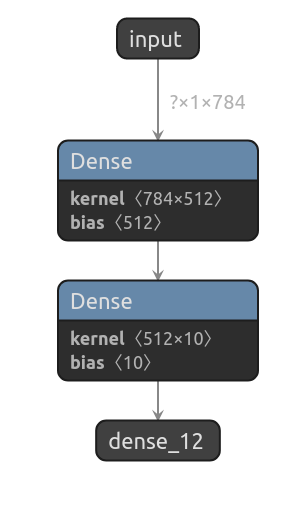
\includegraphics[scale=0.35]{tex/inc/img/keras.png}
        \caption{Keras сеть}
    \end{center}
\end{figure}

\subsubsection{Circle модель}

Поскольку добавленный инструмент работает только с circle моделями, необходимо сконвертировать обученную модель в необходимый формат. Для этого можно воспользоваться уже имеющимся в ONE инструментом tf2circleV2. На рис. 2.3 показан граф этой модели.

\begin{figure}[H]
    \begin{center}
        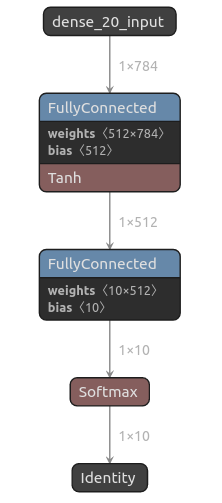
\includegraphics[scale=0.5]{tex/inc/img/circle.png}
        \caption{Circle сеть}
    \end{center}
\end{figure}

\subsubsection{Квантизованная модель}

Для обучения параметров квантизации следует воспользоваться добавленным в этой работе инструментом, однако перед этим необходимо подготовить выборку, которая будет прогоняться через сеть для получения распределения входных параметров. lquantizer позволяет работать с данными в формате hdf5, поэтому перед этим обучающий и валидационный датасеты были преобразованы в этот формат.

Воспользоваться новым инструментом возможно через bash терминал linux при помощи команды с листинга 2.6.

\begin{lstlisting}[language=bash, caption={Пример запуска квантизатора}]
./lquantizer --input_model model.circle  --output_model answer.circle \
             --input_data train.hdf5 --encode_bits 3
\end{lstlisting}

После некоторого ожидания lquantizer создает новый файл с квантизованной моделью, структура которой отражена на рис. 2.4.

\begin{figure}[H]
    \begin{center}
        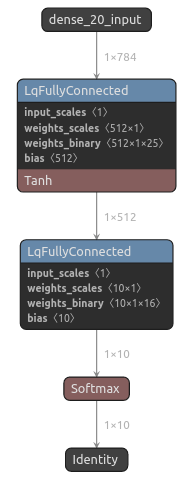
\includegraphics[scale=0.5]{tex/inc/img/lqcircle.png}
        \caption{Квантизованная сеть}
    \end{center}
\end{figure}

% -msse4.2
\subsection{Результаты}

При сравнении моделей основными метриками являются объем памяти, занимаемый сетью, средняя скорость её работы и точность на валидационной выборке, на которой не обучалась ни одна из них. 

\subsubsection{Оценка занимаемой памяти}

Для того, чтобы оценить объем памяти, занимаемый моделью, достаточно посмотреть на вес файла, в котором она хранится. Результаты представлены в таблице 2.1.

\begin{table}[H]
\caption{Занимаемая память исходной и квантизованных моделей}
\begin{center}
\begin{tabular}{|c|c|c|c|c|}
\hline
 -  & fp32 & int3 & int2 & int1 \\
\hline
Объём & 2.1 Mb & 218.3 Kb & 147.2 Kb & 76.2 Kb \\
\hline
\end{tabular}
\end{center}
\end{table}

\subsubsection{Оценка качества обучения}

Чтобы оценить работу алгоритма обучения, следует рассмотреть насколько удачно обучаются уровни квантизации для параметров нейронных слоёв. Гистограмма значений весов и уровни квантизации для случайного нейрона в первом слое рассматриваемой модели отображены на рис. 2.5.

\begin{figure}[H]
    \begin{center}
        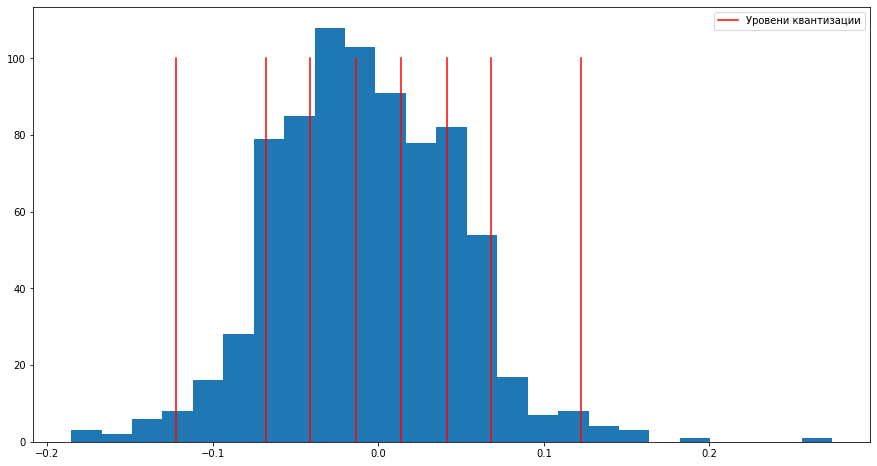
\includegraphics[scale=0.5]{tex/inc/img/firstneuro.png}
        \caption{Распределение весов и уровней квантизации в нейроне}
    \end{center}
\end{figure}


Стоит отметить, что уровни квантизации плотнее расположены к тем значениям весов, которые встречаются в нейроне наиболее часто.

Поскольку датасет, на котором обучалась модель, является сбалансированным, для оценки точности модели можно воспользоваться метрикой Accuracy по формуле (2.1), где $True$ означает количество правильных ответов сети, а $Count$ - количество записей в датасете.

\begin{equation}
Accuracy = \frac{True}{Count}
\end{equation}

Для того, чтобы получать ответы оцениваемых нейронных сетей на валидационной выборке, была написана несложная программа,  которая вызывает в себе luci\_interpreter на данных из hdf5 файла и замеряет время работы каждого вызова. После чего, при помощи скрипта на языке Python подсчитывается значение метрики Accuracy. Результаты проведенных замеров приведены в таблице 2.2.

\begin{table}[H]
\caption{Показатели точности исходной и квантизованных моделей}
\begin{center}
\begin{tabular}{|c|c|c|c|c|}
\hline
 -  & fp32 & int3 & int2 & int1 \\
\hline
Accuracy & 97.19 \% & 95.59 \% & 88.86 \% & 75.11 \% \\
\hline
\end{tabular}
\end{center}
\end{table}

\subsubsection{Оценка производительности}

Оценка производительности производится путем сравнения среднего времени работы нейронных сетей на наборе входных данных. Для этого в программе, реализованной для оценки точности, присутствует опция замера времени работы сети для каждого из входных векторов.

Характеристики ЭВМ, на котором производился запуск:
\begin{itemize}
    \item Операционная система: Ubuntu 18.04.5 LTS
    \item Количество ОЗУ: 16Гб
    \item Процессор: Intel Core i7-8550U CPU @ 1.80GHz × 8 (имеется поддержка SSE 4.2)
    \item Версия компилятора: gcc 7.5.0
\end{itemize}

Чтобы оценить насколько возрастает скорость работы квантизованных сетей при использовании процессорной инструкции POPCNT из набора SSE 4.2, были проведены замеры при стандартной сборке luci\_interpreter и с опцией компилятора -msse4.2. Результаты замеров отображены в таблице 2.3.

\begin{table}[H]
\caption{Производительность исходной и квантизованных моделей}
\begin{center}
\begin{tabular}{|c|c|c|c|c|}
\hline
 -  & fp32 & int3 & int2 & int1 \\
\hline
x86 & \textbf{584.829 мкс} & \textbf{510.210 мкс} & \textbf{256.711 мкс} & \textbf{82.0352 мкс} \\
\hline
SSE 4.2 & \textbf{583.931 мкс} & \textbf{152.743 мкс} & \textbf{84.7845 мкс} & \textbf{44.7829 мкс} \\
\hline
\end{tabular}
\end{center}
\end{table}
